\usetikzlibrary{arrows.meta,calc,fit,matrix,shapes}
\providecommand{\computer}{%
    
\includegraphics[width=1cm]{../common/Noun_project_216.pdf}
}
\providecommand{\computerAlt}{%
    
\includegraphics[width=1cm]{../common/Noun_project_alt_cpu.pdf}
}
\providecommand{\switch}{%
    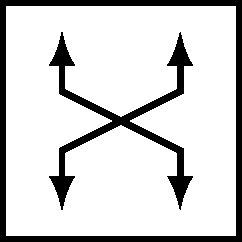
\includegraphics[width=0.9cm]{../common/fig-switch.pdf}
}
\providecommand{\router}{%
    
\includegraphics[width=0.9cm]{../common/fig-router.pdf}
}

\begin{frame}{ARP hijacking}
\begin{tikzpicture}
\tikzset{
    computer/.style={inner sep=0mm,outer sep=0mm,execute at begin node={\computer}},
    computer alt/.style={inner sep=0mm,outer sep=0mm,execute at begin node={\computerAlt}},
    switch/.style={inner sep=0mm,outer sep=0mm,execute at begin node={\switch}},
    router/.style={inner sep=-1mm,outer sep=0mm,execute at begin node={\router},circle},
    connect/.style={draw,very thick,Latex-Latex},
    connect big/.style={draw,ultra thick,Latex-Latex},
    addr label/.style={align=left,font=\fontsize{9}{10}\selectfont\tt},
    arp table/.style={
        tight matrix,
        nodes={minimum height=.6cm},
        column 1/.style={nodes={text width=2.05cm,font=\small\tt}},
        column 2/.style={nodes={text width=1.75cm,font=\small\tt}},
        %row 1/.style={nodes={font=\small}},
    },
    packet/.style={
        draw=blue,very thick,font=\tt\small,
        align=left,
    },
}
\begin{scope}
    \node[computer,label={[addr label]north:MAC 77:\ldots:BB\\IP 10.0.2.2}] (n1-from) at (0, 0) {};
    \node[computer alt,label={[addr label]south:MAC A5:\ldots:BA\\IP 10.0.2.9}] (n1-toA) at (-3, -4) {};
    \node[computer alt,label={[addr label]south:MAC 09:\ldots:FE},font=\Huge] (n1-toB) at (3, -4) {};
    \node[font=\huge] at (n1-toB) {\emoji{smiling-face-with-horns}};
    \node[switch] (sw) at (0, -2) {};
    \draw[connect] (n1-from) -- (sw);
    \draw[connect] (n1-toA) -- (sw);
    \draw[connect] (n1-toB) -- (sw);

    \begin{visibleenv}<2>
    \node[packet,anchor=north west] (blue spoof) at (3, 0) {
        09:\ldots:FE$\rightarrow$77:\ldots:BB \\
        10.0.2.9{\normalfont{} is }09:\ldots:FE
    };
    \node[packet,draw=violet,anchor=north west] (violet spoof) at (-1, -5) {
        09:\ldots:FE$\rightarrow$A5:\ldots:BA \\
        10.0.2.2{\normalfont{} is }09:\ldots:FE
    };
    \draw[blue,line width=1mm,dotted,-Latex] ([yshift=3mm]n1-toB.west) -- ([xshift=1mm]sw.center) -- (n1-from)
        coordinate[midway] (blue spoof point);
    \draw[violet,line width=1mm,dotted,-Latex] ([yshift=1mm]n1-toB.west) --
        ([xshift=-1mm,yshift=-1mm]sw.center) coordinate[midway] (violet spoof point) -- (n1-toA);
    \draw[blue,very thick] (blue spoof) -- (blue spoof point);
    \draw[violet,very thick] (violet spoof) -- (violet spoof point);
    \end{visibleenv}
    \begin{visibleenv}<3>
    \draw[Latex-Latex,red,line width=1mm] ([xshift=1mm]n1-from.south) -- ([xshift=1mm]sw.center)
        -- ([yshift=5mm]n1-toB.west);
    \draw[Latex-Latex,red,line width=1mm] ([yshift=-2mm]n1-toA.north east) -- ([yshift=-2mm]sw.center)
        -- ([yshift=0mm]n1-toB.west);
    \node[align=left,anchor=north west,draw=red,ultra thick] at (2, 0) {
        10.0.2.2 and 10.0.2.9 have \\
        ``poisoned'' ARP tables \\
        makes them send everything to attacker \\
        (instead of each other)
    };
    \end{visibleenv}
    % FIXME: ARP message to 10.0.2.2 with false 10.0.2.9
    % FIXME: ARP message to 10.0.2.9 with false 10.0.2.2
\end{scope}
\end{tikzpicture}
\end{frame}
